%(BEGIN_QUESTION)
% Copyright 2006, Tony R. Kuphaldt, released under the Creative Commons Attribution License (v 1.0)
% This means you may do almost anything with this work of mine, so long as you give me proper credit

Både Bernoullis og Torricellis ligning gir en matematisk sammenheng mellom trykk og strømningsrate. Det betyr at vi kan måle trykk og dermed utlede strømning:

\vskip 10pt

{\bf Differansetrykk som følge av trykkfall over venturi-halsen}:

$$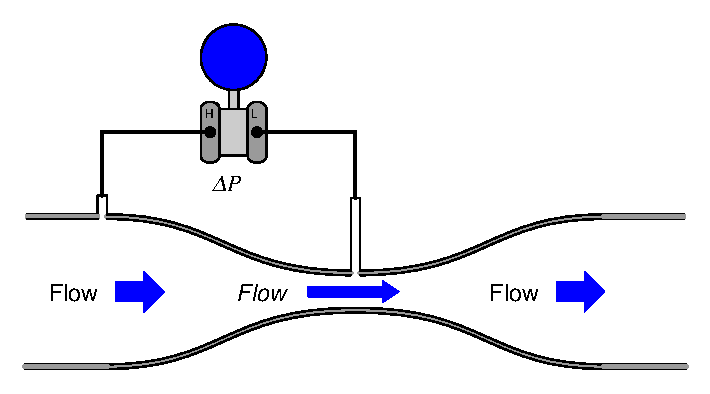
\includegraphics[width=15.5cm]{i00453x01.eps}$$

\vskip 10pt

{\bf Hydrostatisk trykk som følge av væskesøylehøyde}:

$$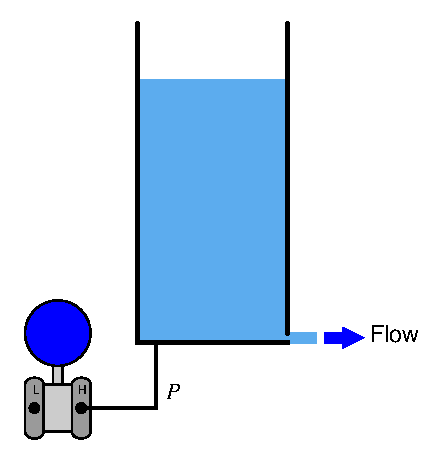
\includegraphics[width=15.5cm]{i00453x02.eps}$$

\vskip 10pt

Utfordringen er at den matematiske sammenhengen i begge disse tilfellene {\it ikke} er lineær. Basert på Bernoullis og/eller Torricellis ligning: Hvilken type sammenheng er dette? Hva må gjøres med signalet fra trykktransmitteren for å få en lineær representasjon av strømning?

\underbar{file i00453}
%(END_QUESTION)





%(BEGIN_ANSWER)

Sammenhengen mellom trykk og strømning er kvadratisk.

%(END_ANSWER)





%(BEGIN_NOTES)

$$P \propto Q^2$$

$$Q \propto \sqrt{P}$$

\noindent
Der,

$P$ = trykk

$Q$ = strømningsrate

\vskip 10pt

%INDEX% Physics, dynamic fluids: relationship between turbulent flow and pressure

%(END_NOTES)
